\section{高亏格视角下的 GW 理论导引 (Patrick Lei)}%
\label{sec:Intro to GW theory with a view to higher genus (Patrick Lei)}


\subsection{GW 理论简介}%
\label{sub:Introduction to GW theory}

关于虚拟基本类的构造，见~\cite{BehrendFantechi1997}；关于公理与量子上同调，见~\cite{KM1994}。

本系列讲座的目标是以一种便于进行高亏格计算的方式讨论 Gromov-Witten 理论。Gromov-Witten 理论研究的是模空间 \(\Mbar_{g,n}(X, \beta)\) 上的积分，其中 \(X\) 是光滑射影代数簇，\(\beta \in H_2(X, \Z)\) 是有效曲线类。有如下图表
\begin{equation*}
\begin{tikzcd}
    \mc{C} \ar{r}{f} \ar[bend right=20]{d}[swap]{\pi} & X \\
    \Mbar_{g,n}(X, \beta) \ar[bend right=20]{u}[swap]{\sigma_i} \ar{ur}[swap]{\on{ev}_i}
\end{tikzcd}
\end{equation*}
其中 \(\mc{C}\) 是万有曲线，\(\sigma_i\) 是 \(\pi\) 的截面，给出标记点，\(f\) 是万有稳定映射，而 \(\ev_i = f \circ \sigma_i\) 是赋值映射。虽然 \(\Mbar_{g,n}(X, \beta)\) 一般是奇异的、不是等维的、也可约的，但存在一个特殊类
\[ [\Mbar_{g,n}(X, \beta)]^{\vir} \in A_{\ab(c_1(X), \beta) + (\dim X - 3)(1-g) + n}(\Mbar_{g,n}(X, \beta), \Q), \]
称为\textit{虚拟基本类}。

\begin{exer}
    用形变理论中的标准论证验证，\(\Mbar_{g,n}(X, \beta)\) 的“期望维数”就是上面给出的数。
\end{exer}

在 \(X\) 光滑射影的假设下，\(\Mbar_{g,n}(X, \beta)\) 是紧的，因此可以定义\textit{GW 不变量}
\[ \ab<\tau_{a_1}(\alpha_1), \cdots, \tau_{a_n}(\alpha_n)>_{g,n,\beta} \coloneqq \int_{[\Mbar_{g,n}(X, \beta)]^{\vir}} \prod_{i=1}^n \ev_i^* \alpha_i \cdot \psi_i^{a_i} \]
其中 \(\alpha_i \in H^*(X)\)。这里，\(\psi_i\) 由 \(\psi_i = c_1(\sigma_i^*(\omega_{\pi}))\) 定义。

遗憾的是，计算单个 Gromov-Witten 不变量非常困难，因此我们将考虑更困难的问题：研究 GW 不变量的生成级数，例如当 \(X\) 是 Calabi-Yau 三维流形时
\[ F_g = \sum_{\beta \geq 0} q^{\beta} \ab<>_{g,0,\beta} \]
其中 \(q\) 是记录曲线类的形式变量，我们将环 \(\Q\ps{q^{\beta} \mid \beta \in H_2(X, \Z)_{\mr{eff}}}\) 记为 \(\Lambda\)。我们还将考虑其他一些结构。首先，可以考虑\textit{量子上同调环}，其乘积 \(a \star_{\mbf{t}} b\) 由公式给出
\[
    (a \star_{\mbf{t}} b, c) = \sum_{\substack{\beta \geq 0 \\ n \geq 0}} \ab<a,b,c, \mbf{t}, \ldots, \mbf{t}>_{0,3+n,\beta} \frac{q^{\beta}}{n!}.
\]
这里 \(a,b,c, \mbf{t} \in H^*(X)\)。我们还将考虑\textit{量子联络}。设 \(\ab\{ e_i \}\) 为 \(H^*(X)\) 的一组基。则量子联络是 \(H^*(X) \times \P^1_z\) 上以 \(H^*(X)\) 为纤维的平凡丛上的联络，由公式给出
\[ \nabla_{t^i} = \partial_{t^i} + \frac{1}{z} e_i \star_{\mbf{t}}. \]
有时，考虑 \(z\) 方向的联络也很有用，其定义为
\[ \nabla_{z \odv{}{z}} \coloneqq z \odv{}{z} - \frac{1}{z} E_X \star_{\mbf{t}} + \mu_X, \]
其中 \(\mu_X(\alpha) = \frac{\deg(\alpha) - \dim X}{2} \alpha\) 是分次算子，而
\[ E_X = c_1(X) + \sum_i \ab(1 - \frac{\deg(e_i)}{2})t^i e_i \]
是\textit{Euler 向量场}。因为我们主要关心 Calabi-Yau 簇，所以不再考虑它。

\subsection{亏格零的计数镜像对称}%
\label{sub:Enumerative mirror symmetry in genus zero}

上世纪 90 年代初，Candelas、de la Ossa、Green 和 Parkes~\cite{CandelasEtAl1991} 通过把问题转化为在另一个称为\textit{镜像五次三维流形}的 Calabi-Yau 三维流形上计算周期积分（等价地，研究其 Hodge 结构的变化），预言了一般五次三维流形上低次有理曲线的条数，这促使数学家发展和研究 Gromov-Witten 理论。在亏格零时，所有不变量都可以从\textit{J-函数} \(J_{\mbf{t}}(q,z) \in H^*(X, \Lambda)[z]\) 恢复，其定义为
\[ \ab( J_{\mbf{t}}(q, z), \alpha ) \coloneqq (z + \mbf{t}, \alpha) + \sum_{n, \beta} \frac{q^{\beta}}{n!} \ab< \frac{\alpha}{z-\psi}, \mbf{t}, \ldots, \mbf{t}>_{0,1+n, \beta} \]
对任意 \(\mbf{t} \in H^*(X, \Lambda)[z]\) 和 \(\alpha \in H^*(X)\) 成立，其中 \((-,-)\) 是 Poincar\'e 配对。因此，计算所有带后代（即 \(\psi\)-类）的亏格零 Gromov-Witten 不变量的问题化为计算 J-函数的问题。

\begin{rmk}
    我们把 \(\frac{1}{z-\psi}\) 展开为 \(\sum_{k=0}^{\infty} \psi^k z^{-k-1}\)。
\end{rmk}

我们应当注意，J-函数可以通过量子微分方程的基本解得到，该基本解由下式给出
\[ ( S_{\mbf{t}}(z) \phi , \alpha) = (\phi, \alpha) + \sum_{n, \beta} \frac{q^{\beta}}{n!} \ab<\frac{\alpha}{z-\psi}, \phi, \mbf{t}, \ldots, \mbf{t}>_{0, 2+n, \beta}. \]
它具有性质 \(S_{\mbf{t}}^*(-z) S_{\mbf{t}}(z) = \on{Id}\)，通常称为\textit{辛性质}。由此，我们可以通过 \(z S_{\mbf{t}}^*(z)\cdot 1 = J_{\mbf{t}}(q, z)\) 恢复 J-函数。

在物理中，镜像对称是两种不同理论（称为 A-模型和 B-模型）之间的对偶，因此我们现在需要引入 B-模型的对象。为了节省时间（和记号），我们假设 \(X\) 是环簇且 \(-K_X\) 是 nef 的。设 \(D_1, \ldots, D_r\) 为 \(X\) 中全体环不变除子。则定义 \(I\)-函数
\[
    I_{\mbf{t}}(q, z) \coloneqq z e^{\mbf{t}/z} \sum_{\beta \geq 0} q^{\beta} \frac{\prod_{i=1}^r \prod_{m = -\infty}^{0} (D_i + mz)}{\prod_{i=1}^r \prod_{m=-\infty}^{\beta \cdot D_i} (D_i + mz)}.
\]
注意这里出现的任何 \((D_i + mz)^{-1}\) 都展开为 \(\frac{1}{mz} \ab(1 - \frac{D_i}{mz} + \cdots)\)，即关于 \(\frac{D_i}{mz}\) 的几何级数。此外，I-函数被一个称为\textit{Picard-Fuchs 方程}的微分方程所零化，该方程是某种超几何型方程。

\begin{exm}
    若 \(\mbf{t} = 0\) 且 \(X = \P^1\)，则得到
    \begin{align*}
        I(q,z) &= z\sum_{d \geq 0} q^d \frac{1}{\prod_{m=1}^d (H + mz)^2} \\
        &= z\sum_{d \geq 0} \ab(\frac{q}{z^2})^d \frac{1}{(d!^2)} + O(H),
    \end{align*}
    因此事实上首项就是第一类 Bessel 函数。
\end{exm}

若 \(X\) 是环簇 \(Y\) 中由线丛 \(L_1, \ldots, L_k\) 截出的完全交，且对 \(Y\) 的任意亏格零稳定映射都有 \(H^1(f^* L_i) = 0\)（这称为\textit{凸}），则量子 Lefschetz 定理~\cite{CoatesGivental2007}允许我们把 \([\Mbar_{g,n}(X, \beta)]^{\vir}\) 替换为 \(e\ab(\bigoplus \pi_* f^* L_i) \cap [\Mbar_{g,n}(Y, \beta)]^{\vir}\)，并在 \(Y\) 上进行所有计算。此时，I-函数定义为
\[
    I_{\mbf{t}}(q,z) \coloneqq z e^{\mbf{t}/z} \sum_{\beta \geq 0} q^{\beta} \frac{\prod_{i=1}^k \prod_{m=-\infty}^{L_i \cdot \beta} (L_i + mz)}{\prod_{i=1}^k \prod_{m=-\infty}^{0} (L_i + mz)} \frac{\prod_{i=1}^r \prod_{m = -\infty}^{0} (D_i + mz)}{\prod_{i=1}^r \prod_{m=-\infty}^{\beta \cdot D_i} (D_i + mz)},
\]
其中我们滥用记号，把 \(L_i\) 与其第一陈类等同起来。

\begin{exm}
    对于由 \(\P^4\) 上 \(\mc{O}_{\P^4}(5)\) 的截面截出的五次三维流形，在 \(\mbf{t} = 0\) 处的 I-函数由下式给出
    \[ I(q,z) = z \sum_{d \geq 0} q^d \frac{\prod_{m=1}^{5d}(5H+mz)}{\prod_{m=1}^d (H+mz)^5}. \]
\end{exm}

亏格零镜像定理的内容就是这两个对象之间的对应。更确切地说，在 \(-K_X\) 为 nef 的情形下，它们由一个变量替换联系起来。

\begin{thm}[{\cite{Givental1998,LLY1997}}]
    把 \(\mbf{t} = 0\) 时的 I-函数写成 \(I_0(q) \cdot z + I_1(q) + O(z^{-1})\)。则有
    \[
        J_{\tau(\mbf{t})}(q,z) = \frac{I_{\mbf{t}}(q,z)}{I_0(q)},
    \]
    其中 \(\tau(\mbf{t}) = \frac{\mbf{t} + I_1(q)}{I_0(q)}\)。
\end{thm}

\begin{exm}
    当 \(X = \P^1\) 时，注意 \(I_0(q) = 1\) 且 \(I_1(q) = 0\)，因此事实上有等式
    \[ J_{\mbf{t}}(q,z) = I_{\mbf{t}}(q,z). \]
\end{exm}

\begin{exm}
    当 \(X\) 为五次三维流形时，为方便起见，我们把 I-函数的分支写成 \(I_0(q) \cdot z + I_1(q)H + O(z^{-1})\)。有
    \[ I_0(q) = \sum_{d \geq 0} \frac{(5d)!}{(d!)^5} q^d, \qquad I_1(q) = \sum_{d \geq 0} \frac{(5d)!}{(d!)^5} \ab(5\sum_{m=d+1}^{5d} \frac{1}{m}) q^d, \]
    因此此时镜像映射是非平凡的。取 \(\mbf{t} = 0\) 的特殊情形，可见 \(\tau = \frac{I_1(q)H}{I_0(q)}\)，于是得到
    \[ J_{\tau}(q,z) = \frac{I(q,z)}{I_0(q)}. \]
    由除子方程，左端也等于 \(J(qe^{I_1/I_0}, z)\)，我们也称之为镜像映射。
    因此，我们可以用镜像定理计算 $\star_{\tau}$。在 \(H^2\) 方向的量子联络变为常微分方程
    \[ (H+zD) S_{\tau}(z)^* = S_{\tau}(z)^* \cdot I_{11} H \star_{\tau}, \]
    其中 $D \coloneqq q \odv{}{q}$（此处坐标为 $\log q$）且 $I_{11} \coloneqq 1 + D \ab(\frac{I_1(q)}{I_0(q)})$。利用镜像定理和 Zagier--Zinger~\cite{ZagierZinger2008} 的结果进行显式计算，得到
    \begin{align*}
        I_{11} H + \cdots &= S_{\tau}(z)^* (I_{11} H \star_{\tau} \1) \\
        \ab( 1 + D\ab(\frac{\frac{I_1}{I_0} + D \ab(\frac{I_2}{I_0})}{I_{11}}) ) H^2 + \cdots &= S_{\tau}(z)^* (I_{11} H \star_{\tau} H) \\
        I_{11} H^3 &= S_{\tau}(z)^* (I_{11}H \star_{\tau} H^2).
    \end{align*}
    因为 $S_{\tau}$ 以恒等映射开头，这就计算出了 $H \star_{\tau}$。
\end{exm}

\subsubsection{振荡积分}%
\label{ssub:Oscillating integrals}

我们现在重新解释亏格零镜像定理，在讨论高亏格不变量时还会回到这一解释。具体而言，我们将把 I-函数解释为 \(X\) 的某个镜像族上的积分，对我们而言该镜像族将是环簇。设
\[ 0 \to \Lambda \to \Z^r \to N \to 0 \]
为 \(X\) 的扇序列。应用 \(\Hom(-, \C^{\times})\)，得到正合列
\[ 1 \to (\C^{\times})^{\dim X} \to (\C^{\times})^r \to \Hom(\Lambda, \C^{\times}) \to 1. \]
假设映射 \(\Lambda \to \Z^r\) 由矩阵 \((m_{ij})_{i=1,\ldots,r}^{j = 1, \ldots, \rho(X)}\) 给出。则考虑簇
\[ E_q = \ab(\prod_{i=1}^r x_j^{m_{ij}} = q_i \middle\vert i=1, \ldots, \rho(X)) \]
它是 \(X\) 的镜像，并考虑超势 \(f = x_1 + \cdots + x_r\)。若要考虑带等变参数 \(\lambda_1, \ldots, \lambda_r\) 的等变理论（分别作用在 \(X\) 的每个齐次坐标上），则考虑 \(f_{\lambda} = \sum_{i=1}^r (x_i - \lambda_i \log x_i)\)。

\begin{exm}
    当 \(X = \P^n\) 时，\(X\) 的镜像是簇 \(E_q = (x_1 \cdots x_{n+1} = q)\) 上的超势 \(\sum_{i=1}^{n+1} (x_i - \lambda_i \log x_i)\)。
\end{exm}

我们现在在（等变）超势的每个临界点 \((x_{\alpha})\) 附近选取适当的 Lefschetz thimble \(\Gamma_{\alpha}\)，并考虑积分
\[ I_{\alpha} = \int_{\Gamma_{\alpha}} e^{f_{\lambda}/z} \prod_{i=1}^r \frac{\d{x_i}}{x_i}. \]
这对应于在 I-函数的表达式中把每个 \(D_i\) 换成 \(D_i - \lambda_i\)（即打开等变参数），在 J-函数中则对应于考虑 \(X\) 的完全等变 GW 理论。在亏格零时，\(\lambda_i \to 0\) 的极限存在，因此可以从下述定理安全地恢复原来的镜像定理：

\begin{thm}[{\cite{Givental1996}}]
    该积分被与 I-函数相同的 Picard-Fuchs 方程所零化，并且在差若干前因子意义下，它沿负实轴当 \(z \to 0^-\) 时的渐近展开，与对应于临界点 \(( x_{\alpha} )\) 的 \(X\) 上 T-不动点所对应的 I-函数的限制一致。
\end{thm}


\subsubsection{拉格朗日锥}%
\label{ssub:The Lagrangian cone}

\(X\) 的量子上同调是\textit{Frobenius 流形}的一个例子，稍后我们会看到它可以由任意上同调场论产生。记 \(V = H^*(X)\)，设 \((e_{\mu})\) 为 \(V\) 的一组基，于是可以写 $\bv = \sum_{\mu,n} t^{\mu}_n e_{\mu} z^n \in V\ps{z}$。
Frobenius 流形的结构来自函数
\[
    \mc{F}_0(\bv) = \sum_{n, \beta, \mu} \frac{q^{\beta}}{n!} \ab<\bv(\psi), \ldots, \bv(\psi)>_{0,n,\beta},
\]
它也称为 \(X\) 的\textit{亏格零后代势}。它满足弦方程、dilaton 方程和拓扑递归关系：
\begin{align*}
    \pdv{}{t_0^1} \mc{F}_0 &= \frac{1}{2} (\bv_0, \bv_0) + \sum_{n=0}^{\infty} \sum_{\mu} t_{n+1}^{\mu} \pdv{}{t_n^{\mu}} \mc{F}_0; \\
    \pdv{}{t_1^1} \mc{F}_0 &= \sum_{n=0}^{\infty} \sum_{\mu} t_n^{\mu} \pdv{}{t_n^{\mu}}\mc{F}_0 - 2 \mc{F}_0; \\
    \pdv{}{t_{k+1}^{\alpha},t_m^{\beta},t_n^{\gamma}} \mc{F}_0 &= \sum_{\mu,\nu} \pdv{}{t_k^{\alpha},t_0^{\mu}} \mc{F}_0 \cdot \eta^{\mu\nu} \cdot \pdv{}{t_0^{\nu},t_{m}^{\beta},t_n^{\gamma}} \mc{F}_0.
\end{align*}
为陈述下述结果，我们考虑无穷维向量空间 $V\ls{z^{-1}}$（或其完备化），其上带有辛形式
\[ \omega(\mbf{f}(z), \mbf{g}(z)) \coloneqq \on{Res}_{z=0}(\mbf{f}(-z), \mbf{g}(z)). \]
我们还引入新变量\footnote{This is called the \textit{dilaton shift}.} $\bq = \bv - z$，于是 \(\mc{F}_0\) 现在是 \(\bq = -z\) 附近的函数。

\begin{thm}[Givental {\cite{Givental2004}}]
    \(\mc{F}_0\) 满足上述偏微分方程当且仅当 \(\d{\mc{F}_0}\) 的图像 \(\mc{L}\) 是以 \(\bq = 0\) 为顶点的 Lagrangian 锥，且其切空间 \(L\) 恰沿 \(zL \subset L\) 与 \(\mc{L}\) 相切。
\end{thm}

我们可以通过如下步骤恢复 Lagrangian 锥 \(\mc{L}\)。先找量子联络的一个基本解
\[ S = \mr{Id} + S_1 z^{-1} + S_2 z^{-2} + \cdots \]
满足方程
\[ z \pdv{}{t^{\mu}}S = e_{\mu} \star S. \]
然后，令 $J \coloneqq z S^*(z) \1$，再按如下步骤恢复 Lagrangian 锥：
\begin{itemize}
    \item 导数 \(\pdv{}{t^{\mu}} J\) 构成 \(L \cap V\ps{z^{-1}}\) 的一组基；
    \item 这蕴含 \(z \pdv{}{t^{\mu},t^{\nu}} J \in L \cap V \ps{z^{-1}}\)。把它们用一阶导数表示，并利用 \(J\) 求解量子联络的事实，即可恢复 Frobenius 结构，从而恢复 Lagrangian 锥。
\end{itemize}

利用这一点，我们可以把亏格零镜像定理解释为：
\begin{thm}[{\cite{Givental1998}}]
    I-函数 \(I_{\mbf{t}}(q,z)\) 落在 \(X\) 的 Lagrangian 锥上。
\end{thm}




\subsection{曲线模空间与上同调场论}%
\label{sub:Moduli of curves and CohFTs}

上同调场论的概念由 Kontsevich--Manin~\cite{KM1994} 引入。

我们把亏格 \(g\) 带 \(n\) 个标记点的稳定曲线的模空间记为 $\Mbar_{g,n}$。它非空当且仅当 \(2g-2+n > 0\)，此时它是维数为 \(3g-3+n\) 的 Deligne-Mumford 叠。全体 \(\Mbar_{g,n}\) 具有组合结构，由一组态射给出。
\begin{itemize}
    \item 有粘合态射
        \[q \colon \Mbar_{g,n+1} \times \Mbar_{h, m+1} \to \Mbar_{g+h,n+m}, \]
        它把两条曲线沿最后一个标记点粘合形成一个节点；
    \item 有自粘合态射 \[s \colon \Mbar_{g-1,n+2} \to \Mbar_{g,n},\]
        它把最后两个标记点粘合起来。
\end{itemize}
当然还有另一个有趣的映射，即遗忘映射
\[ \pr \colon \Mbar_{g,n+1} \to \Mbar_{g,n} \]
它删除最后一个标记点再做稳定化。现在我们可以定义我们感兴趣的计数理论，其中包括 Gromov-Witten 理论。

\begin{defn}
    给定带非退化对称双线性型 \(\eta\) 和单位元 \(\1 \in V\) 的向量空间 \(V\)，\(V\) 上的\textit{上同调场论 (CohFT)} \(\Omega\) 是一族 \(S_n\)-等变的线性映射 \(\Omega_{g,n}\)
    \[ \Omega_{g,n} \colon V^{\otimes n} \to H^*(\Mbar_{g,n}) \]
    满足基本恒等式
    \[ \Omega_{0,3}(\1, u,v) = \eta(u,v) \]
    及如下组合恒等式（设 \(e_{\mu}\) 为 \(V\) 的一组基满足 \(e_1 = \1\)，\(e^{\mu}\) 为对偶基）：
    \begin{align*}
        q^* \Omega_{g+h,n+m}(\bv_1, \bv_2) &= \sum_{\mu} \Omega_{g,n+1}(\bv_1, e_{\mu}) \cdot \Omega_{h,m+1}(  \bv_2, e^{\mu} ); \\
        s^* \Omega_{g,n}(\bv) &= \sum_{\mu} \Omega_{g,n+2}(\bv, e_{\mu}, e^{\mu}).
    \end{align*}
    若还满足恒等式
    \[ \pr^*\Omega_{g,n}(\bv) = \Omega_{g,n+1}(\bv,\1) \]
    则称该 CohFT 具有\textit{平坦单位元}（或满足\textit{弦方程}）。
\end{defn}
所有这些都可以推广到超向量空间，但为简单起见我们不处理这种情形。

\begin{exm}
    CohFT 最重要的例子是光滑射影簇 \(X\) 的 Gromov-Witten 理论。这里，回想稳定映射的源是\textbf{prestable} 曲线，因此有稳定化态射
    \[ \st \colon \Mbar_{g,n}(X,\beta) \to \Mbar_{g,n} \]
    它忘记映射并稳定化曲线。然后，在 Novikov 环上工作，我们取 \(V = H^*(X)\)，\(\eta\) 为 Poincar\'e 配对，\(\1\) 为 \(X\) 的基本类。线性映射 \(\Omega^X_{g,n}\) 由公式给出
    \[ \Omega_{g,n}^X(\btau) \coloneqq \sum_{\beta} q^{\beta} \st_* \ab(\prod_{i=1}^n \ev_i^*(\tau_i) \cap [\Mbar_{g,n}(X,\beta)]^{\vir}), \]
    其中 \(\ev_i \colon \Mbar_{g,n}(X,\beta) \to X\) 是第 \(i\) 个赋值映射。
\end{exm}

\begin{exm}
    设 \(\pi \colon \mc{C}_{g,n} \to \Mbar_{g,n}\) 为万有曲线。则 \textit{Hodge 丛}是向量丛
    \[ \E_{g,n} \coloneqq \pi_* \omega_{\pi}. \]
    我们考虑带通常配对的向量空间 \(V = \C\)，并由公式定义 CohFT \(\Omega^{\E}\)
    \[ \Omega^{\E}_{g,n} \coloneqq c(\E_{g,n}). \]
    粘合公理由等式 \(q^* \E_{g+h} = \E_g \oplus \E_h\) 和正合列
    \[ 0 \to \E_{g-1} \to \E_g \to \mc{O} \to 0. \]
    得到满足。这里，因为亏格零分支对 \(\omega\) 的整体截面没有贡献，且 \(\E\) 不依赖于标记点，该 CohFT 具有平坦单位元。
\end{exm}

\begin{rmk}
    稍后我们会看到，这通过量子 Riemann-Roch 定理与点的 GW CohFT 相关。
\end{rmk}

给定 CohFT \(\Omega\)，可以通过把类 \(\Omega_{g,n}(\bv)\) 与 \(\Mbar_{g,n}\) 上的各种上同调类配对来产生不变量。其中最重要的是一族类
\[ \bar{\psi}_i \coloneqq c_1( s_i^* \omega_{\pi} ), \]
其中 \(s_i \colon \Mbar_{g,n} \to \mc{C}_{g,n}\) 是第 \(i\) 个标记点。

\begin{rmk}
    在 Gromov-Witten 理论中，这些称为\textit{祖先}。还有后代，由同样的公式给出，只是用 prestable 曲线的模空间 \(\mf{M}_{g,n}\) 代替 \(\Mbar_{g,n}\)，其中把上面定义的态射 \(\st\) 分解为
    \[ \Mbar_{g,n}(X,\beta) \xrightarrow{\text{forget map}} \mf{M}_{g,n} \xrightarrow{\text{stabilize}} \Mbar_{g,n}. \]
    后代类记为 \(\psi_i\)。
\end{rmk}

\begin{exm}
    我们计算一个将出现在 Calabi-Yau 三维流形的 GW 理论中的不变量。对任意 CohFT \(\Omega\)，考虑不变量
    \[ \ab<\1\bar{\psi}_1>_{1,1}^{\Omega}\coloneqq \int_{\Mbar_{1,1}} \Omega_{1,1}(\1)\bar{\psi}_1. \]
    利用第二条粘合方程，\(\Omega_{1,1}(\1)\) 的零次部分等于
    \[ \sum_{\mu} \Omega_{0,3}(\1, e_{\mu}, e^{\mu}) = \sum_{\mu} \eta(e_{\mu}, e^{\mu}), \]
    它给出 \(V\) 的（分次）维数 \(\chi(V)\)（例如，若 \(V = H^*(X)\) 其中 \(X\) 为 Calabi-Yau 三维流形，这就是 \(X\) 的拓扑 Euler 示性数）。因此，得到
    \[ \ab<\1\bar{\psi}_1>_{1,1}^{\Omega} = \frac{\dim V}{24}. \]
\end{exm}

\begin{exm}
    考虑点的 GW CohFT。它由 \(V = \C\) 带通常配对及公式
    \[ \Omega_{g,n} = 1. \]
    给出。于是定义不变量
    \[ \ab<\bar{\psi}_1^{a_1} \cdots \bar{\psi}_n^{a_n}>_{g,n} \coloneqq \int_{\Mbar_{g,n}} \Omega_{g,n} \cdot \bar{\psi}_1^{a_1} \cdots \bar{\psi}_n^{a_n}. \]
    \begin{thm}[Kontsevich {\cite{Kontsevich1992}}]
        函数
        \[ \mc{D} \coloneqq \exp \ab(\sum_{g,n} \frac{\hbar^{g-1}}{n!}\sum_{a_1 + \cdots + a_n = 3g-3+n} \ab<\bar{\psi}_1^{a_1} \cdots \bar{\psi}_n^{a_n}>_{g,n} t_{a_1}\cdots t_{a_n}) \]
        被算子
        \begin{align*}
            L_{-1} \coloneqq{}& -\pdv{}{t_0} + \frac{\hbar^{-1}}{2} t_0^2 + \sum_{i=0}^{\infty} t_{i+1} \pdv{}{t_i};\\
            L_0 \coloneqq{}& -\frac{3}{2} \pdv{}{t_1} + \sum_{i=0}^{\infty} \frac{2i+1}{2} t_i \pdv{}{t_i} + \frac{1}{16};\\
            L_n \coloneqq{}& -\frac{(2n+3)!!}{2^{n+1}} \pdv{}{t_{n+1}} + \sum_{i=0}^{\infty} \frac{(2i+2n+1)!!}{(2i-1)!! 2^{n+1}} t_i \pdv{}{t_{i+n}} \\
            &+ \frac{\hbar}{2} \sum_{i=0}^{n-1} \frac{(2i+1) (2i-1) \cdots (2i+1-2n)}{2^{n+1}} \pdv{}{t_i,t_{n-1-i}}.
        \end{align*}
        所零化。
    \end{thm}
\end{exm}

\begin{rmk}
    这一结果（点的 Virasoro 约束）等价于 \(\mc{D}\) 为 KdV 层级的可积 tau-函数，并已被多位作者推广。
\end{rmk}



\subsection{$R$-矩阵作用}%
\label{sub:R-matrix action}

2000 年代初，Givental 发现了公理化计数理论的一个显著性质，即可以用满足性质
\[ R^*(-z) R(z) = \mr{Id}_V. \]
的矩阵 \(R(z) = R_0 + R_1 z + R_2 z^2 + \cdots \in \Hom(V, V')\ps{z}\) 来变换 CohFT。传统文献要求 \(V = V'\) 且 \(R_0 = \mr{Id}\)，但 MSP 学派去掉了这一限制，还允许 \(\dim V < \dim V'\)。

为了定义 \(R\) 在 \(V\) 上定义的 CohFT \(\Omega\) 上的作用，需要回顾 \(\Mbar_{g,n}\) 的一些组合结构。对曲线 \(C\in \Mbar_{g,n}(\C)\)，可以考虑 \(C\) 的对偶图，它有顶点、边和腿，定义如下：
\begin{itemize}
    \item 顶点对应 \(C\) 的不可约分支，并标有一个非负整数，即亏格；
    \item 边对应 \(C\) 的节点（特别地，允许圈）；
    \item 腿对应标记点。
\end{itemize}
任何作为稳定曲线的对偶图出现的图都称为\textit{稳定图}。

\begin{figure}[htpb]
  \centering
  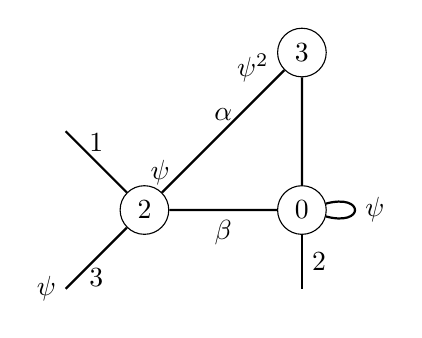
\begin{tikzpicture}[scale=1,transform shape,every loop/.style={}]
    \node[circle,draw] (A) at (0,0) {$2$};
    \node[circle,draw] (B) at (2,2) {$3$};
    \node[circle,draw] (C) at (2,0) {$0$};
    \draw[thick] (A) -- node[above]{$\alpha$} (B) -- (C) -- node[below]{$\beta$} (A);
    \draw[thick] (A) -- node[below]{$3$} (-1,-1);
    \draw[thick] (A) -- node[above]{$1$} (-1,1);
    \draw[thick] (C) -- node[right]{$2$} (2,-1);
    \draw[thick] (C) edge[loop right] node[right] {$\psi$} (C);
    \node[anchor=east] at (-1,-1) {$\psi$};
    \node[anchor=east] at (1.7,1.8) {$\psi^2$};
    \node[anchor=south] at (0.2,0.2) {$\psi$};
  \end{tikzpicture}
  \caption{Example of a stable graph in $\ol{\mc{M}}_{7,3}$ and associated tautological class. This stable graph describes the image of a map
    $\ol{\mc{M}}_{2,4} \times \ol{\mc{M}}_{3,2} \times \ol{\mc{M}}_{0,5} \to \ol{\mc{M}}_{7,3}$.}
  \label{fig:stablegraph}
\end{figure}

CohFT 上的第一类作用是平移作用。设 \(T \in V\ps{z}\)。对 CohFT \(\Omega\)，定义
\[ (T\Omega)_{g,n}(\bv) \coloneqq \sum_m \frac{1}{m!} p_* \Omega_{g,n+m}(\bv, T,\ldots,T) \]
只要该无穷和有意义。

\begin{exm}
    若 \(\Omega^X\) 是光滑射影簇 \(X\) 的 GW CohFT，而 \(\tau \in H^2(X)\) 是除子类，则该无穷和有意义，我们可以定义 \(X\) 的平移后 GW CohFT \(\Omega^{X,\tau}\)。例如，若 \(X\) 是五次三维流形且 \(\tau = \frac{I_1}{I_0} H\)，则平移到 \(\tau\) 就相当于镜像映射 \(q \mapsto Q(q) = q e^{\frac{I_1}{I_0}}\)。
\end{exm}

第二类作用是开头所述的矩阵 \(R\) 的作用。设 \(G_{g,n}\) 表示亏格 \(g\) 带 \(n\) 条腿的所有稳定图的集合。则定义
\[ (R\Omega)_{g,n} \coloneqq \sum_{\Gamma \in G_{g,n}} \frac{1}{\ab|\Aut \Gamma|} \on{Cont}_{\Gamma}, \]
其中 \(\on{Cont}_{\Gamma}\) 由如下构造定义：
\begin{itemize}
    \item 在第 \(i\) 条腿处，放置映射
        \[ R(-\bar{\psi}_i)^* \in \Hom(V',V) \ps{\bar{\psi}_i}; \]
    \item 在每条边处，放置双向量
        \[ V(\bar{\psi}_1, \bar{\psi}_2) \coloneqq \sum_{\mu} \frac{e_{\mu} \otimes e^{\mu} - R(-\bar{\psi}_1)^* e_{\mu} \otimes R(-\bar{\psi}_2)^* e^{\mu}}{\bar{\psi}_1 + \bar{\psi}_2}; \]
    \item 在每个顶点处，放置线性映射
        \[ \Omega_{g_v, n_v} \colon V^{\otimes n_v} \to H^*(\Mbar_{g_v, n_v}); \]
    \item 最后，沿粘合态射 \(\prod_v \Mbar_{g_v, n_v} \to \Mbar_{g,n}\) 考虑上同调中的推出。
\end{itemize}

\begin{defn}
    设 \(R\) 如上。则定义平移
    \[ T_R \coloneqq z (\1 - R(-z)^* \1') \in z V\ps{z}. \]
    只要有意义，就定义
    \[ R.\Omega \coloneqq RT\Omega. \]
\end{defn}

\begin{thm}[Chang-Guo-Li {\cite[Theorem~2.7]{CGL2026}}]
    假设我们在 \(\C\ps{q}\) 系数下工作。则若
    \[ T_R \in z^2 V \ps{z} + zq V \ps{z}, \]
    \(R.\Omega\) 是良定义的 CohFT。此外，若 \(\dim V = \dim V'\)，\(\1'\) 是 \(R.\Omega\) 的单位元。
\end{thm}

关于 \(R_0 \neq \mr{Id}\) 时的平移作用，我们想再多说明一点。为简单起见，假设 \(V = V'\) 且 \(R_0 \1 = c \cdot \1\)，其中 \(c\) 为常数。则置 \(\tilde{T}_R \coloneqq z( \1 - c R(z)^{-1} \1)\)，并利用 dilaton 方程计算
\begin{align*}
    T_R \Omega_{g,n}(\bv) &= \sum_{m=0}^{\infty} \frac{1}{m!} p_*\Omega_{g,n+m}(\bv, T_R, \ldots, T_R) \\
    &= \sum_{k,\ell \geq 0} \frac{1}{k!\ell!} p_* \Omega_{g,n+k+\ell}(\bv, ( (1-c^{-1})\1 \cdot \psi )^{\otimes k}, ( c^{-1} \tilde{T}_R )^{\otimes \ell}) \\
    &= \sum_{k,\ell \geq 0} \frac{(1-c^{-1})^k \cdot c^{-\ell}}{\ell!} \binom{2g-2+n+k+\ell-1}{k} p_* \Omega_{g,n+\ell}(\bv, \tilde{T}_R^{\otimes \ell}) \\
    &= \sum_{m=0}^{\infty} \frac{c^{2g-2+n}}{m!} p_* \Omega_{g,n+m}(\bv, \tilde{T}_R, \ldots, \tilde{T}_R)
\end{align*}
只要这有意义。


\subsection{重构定理}%
\label{sub:Reconstruction theorem}

回想每个 CohFT 都定义了一个 Frobenius 代数。若相应的 Frobenius 代数是半单的，我们称该 CohFT 是\textit{半单}的。

\begin{thm}[Teleman {\cite{Teleman2012}}]%
\label{thm:teleman}
    设 \(\Omega\) 为带平坦单位元的半单 CohFT，\(\omega\) 为其拓扑部分。则存在唯一的
    \[ R = \mr{Id} + R_1 z + \cdots \in \End(V)\ps{z} \]
    使得
    \[ \Omega = R.\omega. \]
\end{thm}

\begin{exm}
    回想之前的 Hodge 丛 CohFT。回想它由公式给出
    \[ \Omega^{\E}_{g,n} = c(\E) = 1 + \lambda_1 + \cdots + \lambda_g. \]
    取零次部分，可见 \(\omega^{\E}\) 就是点的 GW CohFT。利用 Mumford 的计算
    \[ \ch(\E) = g + \sum_{k=1}^{\infty} \frac{B_{2k}}{(2k)!}\ab(\kappa_{2k-1} + \frac{1}{2}\iota_*\sum_{i=0}^{2k-2} \bar{\psi}_1^{i} (-\bar{\psi}_2)^{2k-2-i}), \]
    其中 \(\kappa_{m} = p_* \bar{\psi}_{n+1}^{m+1}\)，\(B_{2k}\) 为 Bernoulli 数，\(\iota\) 是计入 \(2:1\) \'etale 覆盖的边界包含，以及公式
    \[ c(E) = \exp \ab(-\sum_k (-1)^k (k-1)!\ch_k(E)) \]
    对任意向量丛 \(E\) 成立（或直接用量子 Riemann-Roch 定理\footnote{There is a sign error in Coates-Givental, which has propagated to the rest of the literature.}），得到 \(R\)-矩阵
    \[ R(z) = \exp\ab( \sum_{k=1}^{\infty} \frac{B_{2k}}{2k(2k-1)} z^{2k-1}) = 1+\frac{1}{12}z + \cdots. \]

    作为合理性检验，我们用 \(R\)-矩阵计算 \(\Omega_{1,1}^{\E}\)。首先，考虑~\Cref{fig:03graphloop} 中的稳定图。
    \begin{figure}[htpb]
    \begin{center}
    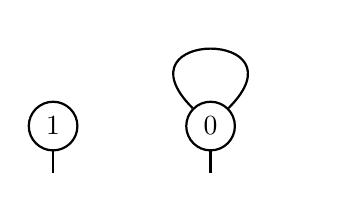
\begin{tikzpicture}[scale=1, transform shape, every loop/.style={}]
    \node[circle,draw=black,thick] (B) at (-1,0) {$1$};
    \draw[-,thick] (B) -- (-1,-0.6);
    \node[circle,draw=black,thick] (A) at (1,0) {$0$};
    \draw[-,thick] (A) -- (1,-0.6);
    \path[every node/.style={font=\sffamily\small},thick]
        (A)   edge[loop] (A);
    \end{tikzpicture}
    \end{center}
    \caption{Stable graphs for $g=1, n=1$}%
    \label{fig:03graphloop}
    \end{figure}
    第一个图 \(\Gamma_1\) 给出的贡献为
    \begin{align*}
        \Cont_{\Gamma_1} &= T\omega_{1,1}^{\E}(R(z)^{-1}\1) \\
        &= \omega_{1,1}^{\E}(R(z)^{-1}\1) + p_* \omega_{1,1}^{\E}(R(z)^{-1}\1, T_R(z)).
    \end{align*}
    利用公式 \(B_2 = \frac{1}{6}\) 以及 \(\dim \Mbar_{1,1} = 1\) 的事实，这变为
    \[ 1 - \frac{1}{12}\psi_1 + \frac{1}{12} \kappa_1. \]
    第二个图没有尾部贡献，因为 \(\dim \Mbar_{0,3} = 0\)。边贡献的常数项为 \(\frac{1}{12}\)，因此考虑自同构并推出到 \(\Mbar_{1,1}\)，得到
    \[ \Cont_{\Gamma_2} = \frac{1}{12} \Delta, \]
    其中 \(\Delta\) 表示边界除子（带正确的叠结构）。因为此时 \(\psi_1 = \kappa_1\)，得到
    \[ 1+\lambda_1 = 1 + \frac{1}{12}(\kappa_1 - \psi_1 + \Delta) = 1 + \frac{1}{12} \Delta. \]
\end{exm}




\subsection{算子形式与几何量子化}%
\label{sub:Operator formalism and geometric quantization}

我们回到 Givental 的辛形式体系。这对某些计算更方便，但事实上在计算生成函数时它与之前的内容是等价的，至少在我们想计算生成函数时如此。回想我们在 \(V\) 上有 Frobenius 流形结构，并考虑了带辛形式的向量空间 \(\mc{V}\coloneqq V\ls{z^{-1}}\)
\[ (\mbf{f}(z), \mbf{g}(z)) \coloneqq \on{Res}_{z=0} \eta(\mbf{f}(-z), \mbf{g}(z)). \]
若考虑由 \(\mc{V}_+ = V[z]\) 和 \(\mc{V}_- = z^{-1}V\ps{z^{-1}}\) 给出的极化，再设 \(\bq\) 如前（带 dilaton 平移），设 \(\bp\) 为 \(\mc{V}_-\) 上的坐标，使得 \((\bq, \bp)\) 构成 \(\mc{V}\) 的一组 Darboux 坐标。

\begin{defn}
    我们把任何形如
    \[ \mc{D} = \exp\ab(\sum_{g=0}^{\infty} \hbar^{g-1} \mc{F}_g) \]
    的形式函数称为 \textit{Fock 空间的渐近元}。
\end{defn}

然后，给定 Fock 空间的这样一个渐近元，我们用如下公式量子化 \(\mc{V}\) 上的（无穷小）辛变换：
\[ \wh{p_a p_b} \coloneqq \hbar \partial_{q_a} \partial_{q_b}, \qquad \wh{p_a q_b} \coloneqq q_b \partial_{q_a}, \qquad \wh{q_a q_b} = \frac{q_a q_b}{\hbar}. \]
特别地，这让我们能理解像 \(\hat{R} \mc{D}\) 这样的表达式。但需小心，因为我们的公式同时涉及基本解 \(S_{\tau}\) 和 \(R\)-矩阵，而 \(S_{\tau}\) 是 \(z^{-1}\) 的幂级数。\footnote{This is because we expand $\frac{1}{z-\psi} = \sum_{n=0}^{\infty} \psi^n z^{-n-1}$.}

\begin{thm}[Givental {\cite{Givental2001quantization}}]
    形如 \(S(z^{-1}) = \mr{Id} + S_1 z^{-1} + \cdots\) 的算子在 Fock 空间的（渐近）元上的作用由公式给出
    \[ \hat{S}^{-1} \mc{D}(\bq) = e^{\frac{1}{2\hbar}W(\bq,\bq)} \mc{D}([S \bq]_+), \]
    其中 \(W = \sum \eta(W_{mn}q_m, q_n)\) 由公式定义
    \[ \frac{S(w^{-1})^* S(z^{-1}) - \mr{Id}}{w^{-1}+z^{-1}} = \sum \frac{W_{mn}}{w^m z^n}. \]
    形如 \(R(z) = \mr{Id} + R_1 z + \cdots\) 的算子作用由公式给出
    \[ \hat{R}\mc{D}(\bq) = e^{\frac{\hbar}{2} V(\partial_{\bq}, \partial_{\bq})} \mc{D}(R^{-1} \bq), \]
    其中 \(V = \sum \eta(p_m, V_{mn} p_n)\) 由
    \[ \frac{R(w)^* R(z) - \mr{Id}}{w+z} = \sum V_{mn} w^m z^n. \]
    定义。
\end{thm}

对半单 CohFT，有一组\textit{典范坐标} \(u_{\alpha}\)，使得 \(1\)-形式 \(\d{u}\) 是代数同态 \(T_v V \to \C\)。于是，在半单点附近，量子联络有形如
\[ \Psi \cdot  R \cdot e^{\frac{U}{z}}, \]
的渐近解，其中 \(\Psi\) 从平坦坐标切换到典范坐标，\(U = \on{diag}(u_{\alpha})\) 是典范坐标矩阵。最后，定义
\[ C = \frac{1}{2} \int^u \sum R_1^{\alpha\alpha} \d{u_{\alpha}}. \]
Teleman 重构定理的一个推论是公式
\[ \mc{D}^X = e^{C(u)} \hat{S}^{-1}_{\tau} \hat{\Psi} \hat{R} \wh{e^{\frac{U}{z}}} \prod_{i=1}^{\dim V} \mc{D}^{\mr{pt}} \]
它对任何具有半单量子上同调的光滑射影簇的 Gromov-Witten 理论成立。

\begin{exm}
    作为最后一个例子，我们用 Teleman 定理计算任意半单 CohFT 的 \(F_1\)。设 \(e_{\mu}\) 表示量子乘积的幂等基。我们计算
    \[ \int_{\Mbar_{1,1}} \Omega_{1,1}(e_{\beta}). \]
    利用重构定理，得到
    \begin{align*}
        \int_{\Mbar_{1,1}}\Omega_{1,1}(e_{\beta}) ={}& \int_{\Mbar_{1,1}} T_R \omega_{1,1}(R(\bar{\psi})^{-1} e_{\beta}) + \frac{1}{2} T_R \omega_{0,3}(R(\bar{\psi})^{-1} e_{\beta}, V(\bar{\psi}_2, \bar{\psi}_3)) \\
        ={}& \int_{\Mbar_{1,1}}T_R\omega_{1,1}(e_{\beta}) - \int_{\Mbar_{1,1}} T_R \omega_{1,1}(R_1 e_{\beta})\bar{\psi} \\ 
        &+ \frac{1}{2}\sum_{\mu}  \omega_{0,3}(e_{\beta}, R_1 e^{\mu}, e_{\mu}) \\
        ={}& \int_{\Mbar_{1,1}} ( \omega_{1,1}(e_{\beta}) + p_* ( \omega_{1,2}(e_{\beta}, R_1 \1) \bar{\psi}_2^2 )) \\
        &- \int_{\Mbar_{1,1}} (\omega_{1,1}(R_1 e_{\beta})\bar{\psi}_1 + p_* ( \omega_{1,2}(R_1 e_{\beta}) \bar{\psi}_2^2 ) \bar{\psi}_1) \\
        &+ \frac{1}{2} \sum_{\mu} \eta(e_{\beta} \star e_{\mu}, R_1 e^{\mu}) \\
        ={}& \frac{1}{24} \sum_{\mu} ( \omega_{0,4}(e_{\mu}, e^{\mu}, e_{\beta}, R_1 \1) -\omega_{0,3}(e_{\mu}, e^{\mu}, R_1 e_{\beta}) )\\
        &+ \frac{1}{2} \eta(e_{\beta}, R_1 e^{\beta}) \\
        ={}& \frac{1}{24} \sum_{\mu}\sum_{\nu} \omega_{0,3}(e_{\mu}, e^{\mu}, e_{\nu})\omega_{0,3}(e^{\nu}, e_{\beta}, R_1 \1) \\
        &-\frac{1}{24} \sum_{\mu} \omega_{0,3}(e_{\mu}, e^{\mu}, R_1 e_{\beta}) + \frac{1}{2} (R_1)_{\beta\beta} \\
        ={}& \frac{1}{24} \ab(\eta(e^{\beta}, R_1 \1) - \sum_{\mu} \eta(e^{\mu}, R_1 e_{\beta})) + \frac{1}{2} (R_1)_{\beta\beta}.
    \end{align*}
    利用恒等式
    \begin{align*}
        \eta(R_1 \1, e^{\beta}) - \sum_{\mu} \eta(R_1 e_{\beta}, e^{\mu}) &= \sum_{\mu} \Delta_{\mu} \int_{\Mbar_{0,4}} \Omega_{0,4}(e_{\mu}, e_{\mu}, e_{\mu}, e_{\beta}) \\
        &= -\frac{1}{2}\sum_{\mu} \Delta_{\mu} \partial_{u_{\beta}} \Delta_{\mu}^{-1} \\
        &= \frac{1}{2} \sum_{\mu} \partial_{u_{\beta}} \log \Delta_{\mu},
    \end{align*}
    其中 \(\Delta_{\mu} \coloneqq \eta(e_{\mu}, e_{\mu})^{-1}\)，得到结果
    \[ \int_{\Mbar_{1,1}} \Omega_{1,1}(e_{\beta}) = \frac{1}{48} \sum_{\mu} \partial_{u_{\beta}} \log \Delta_{\mu} + \frac{1}{2} (R_1)_{\beta\beta}, \]
    它可以写成 suggestive 的形式
    \[ \d{F_1^{\Omega}} = \sum_{\mu} \ab( \frac{\d{\log \Delta_{\mu}}}{48} + \frac{1}{2} (R_1)_{\mu\mu} \d{u_{\mu}} ). \]
    这恢复了 Givental 已知的结果。
\end{exm}

\subsection{如何计算 R-矩阵}%
\label{sub:How to compute the R-matrix}

最后，我们解释如何计算 R-矩阵，先从 Frobenius 流形是共形的情形开始（例如光滑射影簇的 Gromov-Witten 理论、\(r\)-spin 曲线等）。在这个例子中，我们沿用~\cite{PPZ2015} 考虑 3-spin 曲线的 Frobenius 流形。设 \(V\) 是 2 维的，坐标为 \(x\) 和 \(y\)，其中 \(x\) 对应单位元。度量由下式给出
\[ \eta = \begin{pmatrix}
    0 & 1 \\
    1 & 0
\end{pmatrix} \]
而原始亏格零势为 \(F(x,y) = \frac{1}{2} x^2 y + \frac{1}{72} y^4\)。有 \textit{Euler 向量场}
\[ E = x \pdv{}{x} + \frac{2}{3} y \pdv{}{y}, \]
它在 \(\partial_x\) 和 \(\partial_y\) 上的权分别为 \(-1\) 和 \(-\frac{2}{3}\)。共形维数为 \(\delta = \frac{1}{3}\)，我们定义次数算子
\[ \mu(v) = [E,v] + \ab(1 - \frac{\delta}{2})v. \]
这里，\(\partial_x\) 的次数为 \(-\frac{1}{6}\)，\(\partial_y\) 的次数为 \(\frac{1}{6}\)。

为简化计算，置 \(\phi = \frac{y}{3}\) 并定义
\[ \hat{\partial}_x = \phi^{1/4} \partial_x, \qquad \hat{\partial}_y = \phi^{-1/4} \partial_y, \]
然后在此标架下计算。在此情形下，量子乘法由下式给出
\[ \hat{\partial}_x \star \hat{\partial}_x = \phi^{1/4} \hat{\partial}_x, \qquad \hat{\partial}_x \star \hat{\partial}_y = \phi^{1/4} \hat{\partial}_y, \qquad \hat{\partial}_y \star \hat{\partial}_y = \phi^{1/4} \hat{\partial}_x. \]
我们需要的最后一件事是，与 \(E\) 的量子乘法由下式给出
\[ E \star - = \begin{pmatrix}
    x & 2 \phi^{3/2} \\
    2 \phi^{3/2} & x 
\end{pmatrix}. \]
我们现在用递归方程计算 R-矩阵 \(R = 1 + R_1 z + \cdots\)
\[ [R_{k+1}, E \star -] = (k + \mu) R_k. \]
置 \(R_k = \begin{psmallmatrix}
    a_k & b_k \\
    c_k & d_k
\end{psmallmatrix}\)，得到方程
\[ \ab[
    \begin{pmatrix}
        a_{k+1} & b_{k+1} \\
        c_{k+1} & d_{k+1}
    \end{pmatrix}, \begin{pmatrix}
        x & 2 \phi^{3/2} \\
        2 \phi^{3/2} & x 
    \end{pmatrix}
] = \frac{1}{6} \pdiagmat[empty={}]{6k-1, 6k+1} \begin{pmatrix}
    a_k & b_k \\
    c_k & d_k 
\end{pmatrix}. \]

其唯一解事实上为
\begin{align*}
    a_k &= \frac{1}{1728^k \phi^{3k/2}} \frac{1+6k}{1-6k} \frac{(6k)!}{(3k)!(2k)!} \delta_{k, \text{even}},  \\
    b_k &= \frac{1}{1728^k \phi^{3k/2}} \frac{1+6k}{1-6k}\frac{(6k)!}{(3k)!(2k)!} \delta_{k, \text{odd}},  \\
    c_k &= \frac{1}{1728^k \phi^{3k/2}}\frac{(6k)!}{(3k)!(2k)!} \delta_{k, \text{odd}}, \\
    d_k &= \frac{1}{1728^k \phi^{3k/2}} \frac{(6k)!}{(3k)!(2k)!} \delta_{k, \text{even}}. 
\end{align*}
如果你熟悉曲线模空间上的 tautological 关系，就会看到级数 \(a_k + b_k\) 和 \(c_k + d_k\) 出现在 Faber-Zagier 关系和 Pixton 关系的表述中。

在 Frobenius 流形不是共形的情形（例如等变 Gromov-Witten 理论），需要用振荡积分或其他技巧来固定 R-矩阵的初值。我们在此给出一个例子计算，它归功于 Givental~\cite{Givental2001semisimple}。在此情形下 \(X = \P^n\)，但论证可对任何 Fano 环簇成立。回想 \(\P^n\) 的等变镜像是超势
\[ W = x_1 + \cdots + x_{n+1} + \sum_{i=1}^{n+1} \lambda_i \log x_i \]
（此处为方便起见改变了等变参数的符号）。因此，振荡积分形如
\[ I = \int_{\Gamma \subset E_q = (x_1 \cdots x_{n+1}=q)} e^{W/z} \prod_{i=1}^{n+1} \frac{\d{x_i}}{x_i}. \]
它被算子
\[ \prod_{i=1}^{n+1}\ab(zq \odv{}{q} -\lambda_i) - q, \]
所零化，这正是射影空间的 I-函数满足的 Picard-Fuchs 方程。

为在临界点附近展开该积分，首先需要计算临界点。这里，用坐标 \(t = \log q\) 和 \(T_i = \log x_i\)，得到方程
\[ x_i = L - \lambda_i, \]
其中 \(L\) 是 Lagrange 乘子。它们满足方程
\[ \prod_{i=1}^{n+1} (L - \lambda_i) = q, \]
因此对一般的 \(\lambda\) 值，在 \(q = 0\) 附近，Lagrange 乘子的可能取值 \(L_i\) 由它们起始于哪个 \(\lambda_i\) 来区分。注意函数 \(W\)、Lagrange 乘子的值以及临界点都连续依赖于 \(\lambda\)，因此当 \(q \neq 0\) 时它们在 \(\lambda = 0\) 处有非等变极限。

当 \(q = 0\) 时，矩阵 \(\Psi\) 从平坦基 \(\ab{H^i}\) 过渡到基
\[ L_i(H) = \prod_{j \neq i} \frac{H - \lambda_j}{(\lambda_i - \lambda_j)^{1/2}}, \]
它们是典范坐标的首项（只需通过等变局部化计算环作用的不动点，就会得到这个 Lagrange 插值）。因此，需要在 \(q = 0\) 极限下计算 \(L_j \ab(z q \odv{}{q}) I\)。直接计算表明，把 \(L_i \ab(z q \odv{}{q})\) 作用到积分上会在振荡积分的被积函数中引入一个正比于 \(\frac{q}{x_i}\) 的额外因子。因为可以置换指标，我们只计算 \(i = n+1\) 的情形。另一直接计算表明，该积分在 \(q = 0\) 处除非 \( j = n+1\) 否则为零，因此事实上可见 \(R\) 在经典极限下是对角的。当 \(j = n+1\) 时，有
\[ \frac{q}{x_{n+1}} = x_1 \cdots x_n, \]
积分变为
\[ \int_{\Gamma} e^{\ab( \sum_{i=1}^n x_i + (\lambda_i - \lambda_{n+1})\log x_i ) / z} \d{x_1} \cdots \d{x_n} = \prod_{i=1}^n \int_{\R} e^{x_i/z} x_i^{(\lambda_i - \lambda_{n+1})/z} \d{x_i}, \]
它就是 gamma 函数的乘积。

\begin{lem}
    有渐近式
    \[ \log \Gamma(1+s) \sim s \log \ab(\frac{s}{e}) + \frac{1}{2} \log(2\pi s) + \sum_{k=1}^{\infty} \frac{B_{2k}}{2k} \frac{s^{1-2k}}{2k-1}. \]
\end{lem}
利用这一点，可见在 \(q = 0\) 处，R-矩阵的对角元由下式给出
\[ \log R = \sum_{k=1}^{\infty} \frac{B_{2k}}{2k} \frac{z^{2k-1}}{2k-1} \sum_{i =1}^n (\lambda_i - \lambda_{n+1})^{1-2k}. \]
由 Givental 的一个结果，这蕴含该 R-矩阵恢复了 \(\P^n\) 的等变 GW 理论，作为推论，因为非等变极限存在，得到了 \(\P^n\) 的 Virasoro 约束。
